%%%%%%%%%%%%%%%%%%%%%%%%%%%%%%%%%%%%%%%%%
%
% (c) 2022 by Jennifer Laaser
%
% This work is licensed under the Creative Commons Attribution-NonCommercial-ShareAlike 4.0 International License. To view a copy of this license, visit http://creativecommons.org/licenses/by-nc-sa/4.0/ or send a letter to Creative Commons, PO Box 1866, Mountain View, CA 94042, USA.
%
% The current source for these materials is accessible on Github: https://github.com/jlaaser/pogil-polymers
%
%%%%%%%%%%%%%%%%%%%%%%%%%%%%%%%%%%%%%%%%%

\renewcommand{\figpath}{content/polymchem/livingpolyms/ATRP/figs}
\renewcommand{\labelbase}{ATRP}

\begin{activity}{Atom Transfer Radical Polymerization}

\begin{instructornotes}
	This activity introduces students to concepts related to controlled radical polymerization via atom transfer radical polymerization (ATRP).
	
	After completing this activity, students will be able to:
	\begin{enumerate}
		\item Identify the key similarities and differences between ATRP and conventional free-radical polymerizations		
		\item Explain what criterion must be met for ATRP to produce well-controlled (low dispersity) polymers, and relate this criterion to the equilibrum constant of the ATRP reaction
		\item Predict the structure of a polymer produced by a given ATRP reaction
	\end{enumerate}
	
	\subsection*{Activity summary:}
	\begin{itemize}
		\item \textbf{Activity type:} Learning Cycle
		\item \textbf{Content goals:} See above
		\item \textbf{Process goals:} %https://pogil.org/uploads/attachments/cj54b5yts006cklx4hh758htf-process-skills-official-pogil-list-2015-original.pdf
			\begin{itemize}
				\item Reading and interpreting reaction mechanisms
				\item Interpreting mathematical equations
				\item Oral and written communication of reasoning
			\end{itemize}
		\item \textbf{Duration:} 45 minutes, including class discussion
		\item \textbf{Instructor preparation required:} none beyond knowledge of relevant content
		\item \textbf{Related textbook chapters:}
			\begin{itemize}
				\item \emph{Polymer Chemistry} (Hiemenz \& Lodge), 2nd ed.: section 4.6
				\item \emph{Introduction to Polymers} (Young \& Lovell), 3rd ed.: section 4.5.2
			\end{itemize}
		%\item \textbf{Facilitation notes:}
		%	\begin{itemize}
		%		\item \dots
		%	\end{itemize}
	\end{itemize}
	
\end{instructornotes}


\begin{model}[Key Reactions in ATRP]
	\label{\labelbase:mdl:ATRPrxns}

	Atom transfer radical polymerization (ATRP) is a popular method for obtaining narrow molecular weight distributions in radical polymerizations.  The key reactions involved in ATRP are:
	
	\centerline{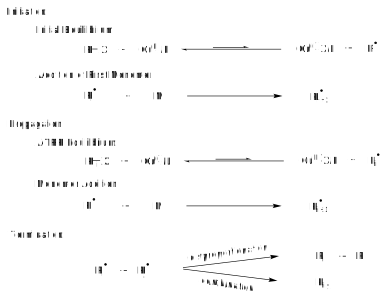
\includegraphics[width=\textwidth]{\figpath/Model1_scheme}}
	
	Here, ``RX'' is an alkyl halide initiator, ``Cu\textsuperscript{(I)}/L'' is a copper-based catalyst, ``M'' is the monomer, and the ``P$_i^\bullet$'' are the propagating chains of length $i$.
	
\end{model}


\begin{ctqs}

	\question Achieving a truly ``living'' polymerization requires there to be no irreversible termination reactions.
	
		\begin{enumerate}
		
			\item Is this criterion strictly obeyed for the reaction scheme shown in Model \ref{\labelbase:mdl:ATRPrxns}?  Why or why not?  \label{\labelbase:ctq:terminationsuprression}
			
				\begin{solution}[1.25in]{}
				
					No, it is not.  The radicals can still terminate by irreversible disproportionation or combination reactions.
					ATRP is thus not truly a \emph{living} polymerization; while some people do still refer to it as a living radical polymerization, it is much more appropriately described as either a \emph{controlled} radical polymerization (commonly used term) or a \emph{reversible-deactivation} radical polymerization (IUPAC preferred).
				
				\end{solution}
			
			\item Recall that in radical polymerizations, the termination rate is given by
				\begin{equation*}\
					R_t = 2k_t[\text{P}^\bullet]^2
				\end{equation*}
				What needs to be true about the concentration of active radicals, [P$^\bullet$], to keep this termination rate as low as possible?
				
				\begin{solution}[0.9in]{}
				
					The concentration of active radicals needs to be kept very low.
				
				\end{solution}
			
		\end{enumerate}
	
	\question The key equilibrium that determines the active radical concentration is the ATRP equilibrium,
	
	\centerline{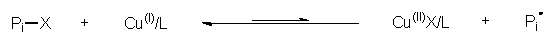
\includegraphics[width=0.7\textwidth]{\figpath/Model1_KATRP_norateconsts}}
		
		\begin{enumerate}
			\item Based on your answer to the previous question, does achieving good control over the molecular weight of polymers synthesized by ATRP require this reaction to favor the left side or the right side of the reaction?
			
				\begin{solution}[0.9in]{}
				
					The equilibrium should favor the left side of the reaction to minimize the concentration of active radicals.
				
				\end{solution}
			
			\item What must be true about the value of the equilibrium constant for this reaction, $K_{ATRP}$, if you want to control the molecular weight of polymers synthesized by ATRP?
			
				\begin{solution}[0.9in]{}
				
					For the left side of the reaction to be favored,  we need to have $K_{ATRP}< 1$ (ideally, $K_{ATRP}\ll 1$)!
				
				\end{solution}
			
		\end{enumerate}

\end{ctqs}

\begin{infobox}
	The structures of several popular ligands used to make catalysts for ATRP, and the ATRP equilibrium constants of the resulting catalysts, are:
	
	\centerline{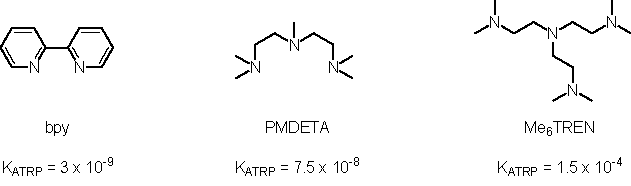
\includegraphics[width=0.8\textwidth]{\figpath/ATRP_ligands}}
\end{infobox}

\begin{ctqs}
	
	\question Which ligand would you expect to give the best dispersity in an ATRP reaction?  Briefly explain your group's reasoning in 1-2 complete sentences.
	
		\begin{solution}[1.25in]{}
		Based solely on the information given above, bpy should give the best dispersity because it has the lowest equilibrium constant.
		
		Note: here we focus only on the equilibrium constant, but as discussed in Exercise \ref{\labelbase:exc:kinetics}, the kinetics of activation and deactivation do matter too.
		\end{solution}
	
	\question If you use a ligand that has \emph{too high} of a value of $K_{ATRP}$, what do you expect to happen to the dispersity of the polymer chains?  Suggest one change you could make to the reaction conditions to mitigate this problem.
	
		\begin{solution}[1.25in]{}
			A very high value of $K_{ATRP}$ would result in a high concentration of active radicals, which would increase the dispersity by increasing the probability of irreversible termination.
			
			To mitigate this problem, we could add Cu\textsuperscript{(II)}X/L to help push the ATRP equilibrium back to the left and decrease the active radical concentration.
		\end{solution}
	
	\question If you use a ligand that has \emph{too low} of a value of $K_{ATRP}$, what do you expect to happen to the overall polymerization rate?  Suggest one change that you could make to the reaction conditions to mitigate this problem. \label{\labelbase:ctq:lowK}
	
		\begin{solution}[1.25in]{}
			The polymerization rate, $R_p$, depends on the concentration of active radicals as $R_p = k_p[\text{M}][\text{P}^\bullet]$.
			
			If $K_{ATRP}$ is too low, then $[\text{P}^\bullet]$ may be so low that the polymerization is very slow.  To address this problem, we could either switch ligands or add more catalyst (both of which would increase the active radical concentration and speed up the polymerization at the cost of worse control over dispersity), or increase the reaction temperature to increase the polymerization rate (although changing the reaction temperature may also affect the equilibrium constant).
		\end{solution}
	
	\question All of the ligands shown above contain nitrogen centers that coordinate to the Cu\textsuperscript{(I)} species to form the active catalyst.
	
		Why might monomers containing primary, secondary, or tertiary amines in their sidechains be difficult to polymerize by ATRP?  
	
		\begin{solution}[1.25in]{}
			Amines in the monomers might complex with the Cu species and change $K_{ATRP}$.
			
			Generally speaking, ATRP works well for monomers containing hydroxyl, epoxide, allyl, and amide functional groups, but is challenging with monomers containing functional groups that can coordinate with the metal center, such as 1$^\circ$, 2$^\circ$, or 3$^\circ$ amines and carboxylic acids.
		\end{solution}
	
\end{ctqs}

\begin{infobox}
	One popular initiator for ATRP is ethyl 2-bromoisobutyrate, or EBriB.  Its structure is shown below:
	
	\centerline{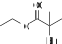
\includegraphics[width=0.15\textwidth]{\figpath/EBriB}}
\end{infobox}

\begin{ctqs}
	\question Draw the structure of the active radical R$^\bullet$ that you expect to be formed when this intiator is activated by the copper catalyst (\emph{hint: remember that the ``X'' in ``RX'' is a stand-in for a halogen atom}): \label{\labelbase:ctq:ATRPinit}
	
		\begin{solution}[0.5in]{}
			\centerline{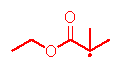
\includegraphics[width=0.2\textwidth]{\figpath/EBriB_radical}}	
		\end{solution}
	
	\question Draw the structure that would be formed if this radical attacks a methyl methacrylate monomer (that is, draw RM$^\bullet$, where the monomer M is methyl methacrylate). \label{\labelbase:ctq:ATRPprop}
	
		\begin{solution}[1in]{}
			\centerline{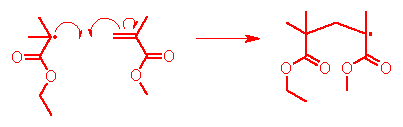
\includegraphics[width=0.5\textwidth]{\figpath/MMA_propagation}}	
		\end{solution}
	
	\question Compare the types of radicals you drew in both of the preceding questions.
	
		\begin{enumerate}
			\item Do you expect EBriB to be a a ``good'' initiator for methacrylate monomers?  Why or why not?  Explain your group's reasoning in 2-3 complete sentences.
	
			\begin{solution}[1.25in]{}
				Yes, EBriB should be a good initiator for methacrylate monomers.  Because they form essentially identical radical centers, the equilibrium constants for the initial equilibrium and ATRP equilibrium should be similar, which helps ensure that all of the initiator molecules will be likely to activate before any of the chains get too long.
				
				Strictly speaking, ensuring that all chains activate ``at once'' (as required for a living polymerization) would require the equilibrium constant for the initial equilibrium to be higher than that for the ATRP equilibrium, but in practice, having these be roughly equal works well enough.
			\end{solution}
			
			\item Based on your response to the previous question, propose a strategy that you could use to choose an initiator based on the structure of the monomer you want to polymerize.
	
			\begin{solution}[1.25in]{}
			
				Generally speaking, we should choose an initiator that will produce a radical with a similar structure to the propagating radical that will be formed from whatever monomer we are polymerizing.
			
			\end{solution}
			
		\end{enumerate}
		
	\question If all goes well, at the end of an ATRP reaction, we isolate (or collect) the ``deactivated'' form of the polymer, $\text{P}_i^\bullet\text{-X}$.
	
		\begin{enumerate}
			\item Draw the structure of the polymer that you would expect to collect at the end of the polymerization started in CTQ \ref{\labelbase:ctq:ATRPprop}.
				
				\begin{solution}[1.5in]{}
			\centerline{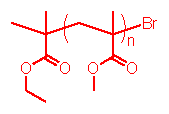
\includegraphics[width=0.25\textwidth]{\figpath/MMA_polym_final}}		
				\end{solution}
			
			\item Based on the structure you drew in response to the preceding question, critique or defend the following statement in 2-3 complete sentences:
			
				\emph{``The polymer collected at the end of an ATRP reaction could be used as an initiator for another ATRP reaction.''}
				
				\begin{solution}[2in]{}
				
					This statement is correct. The polymer produced in an ATRP reaction contains a halogen atom that can be re-activated by an appropriate ATRP catalyst and used as an initiator in another ATRP reaction.  In effect, the whole polymer chain is the ``R'' group on the initiator.
					
					This characteristic of polymers produced by ATRP is particularly useful for synthesis of block copolymers - if the second reaction is performed using a a different monomer than the first reaction, a block copolymer will be formed.
				
				\end{solution}
				
		\end{enumerate}
		
		% NOTE TO SELF: Ideally, I'd really like to get at the issue of the initial vs. ATRP equilibria and which one  needs to have a higher equilibrium constant.  Maybe also look at equilibrium constants for some of the initiators, and get at the difference between Br and Cl
		
		% I'd also like to have a question that gets at the fact that ATRP maintains high chain-end functionality - this is really critical for e.g. synthesis of block copolymers
		
		% these could go in the exercises?  Or, I could have an extension that delves more deeply into ATRP?
		
\end{ctqs}


\begin{exercises}

	\exercise ATRP is often referred to as a ``living radical polymerization''.  Is this term strictly accurate?  Why or why not?  Based on your answer, why do you think some polymer scientists prefer to call ATRP a \emph{controlled} radical polymerization rather than a living radical polymerization?
	
		\emph{Hint: you might want to revisit your answer to CTQ \ref{\labelbase:ctq:terminationsuprression}.}
		
		\begin{solution}{}
			No, ATRP is not truly a living polymerization, because irreversible termination reactions are still possible (even if they are somewhat suppressed).  Controlled radical polymerization is a more appropriate term because it reflects the idea that suppressing the active radical concentration improves our control over the molecular weight distribution of the polymers, even if it does not make the reaction a truly living polymerization.
		\end{solution}		
		
	\exercise 
	
		\begin{enumerate}
	
			\item Which species (initiator, catalyst, or monomer) determines the number of polymer chains formed in an ATRP reaction?
		
		\begin{solution}{}
			The initiator determines the number of chains formed (it is the only one of these three components that can be ``turned into'' an active radical.
		\end{solution}
	
			\item Suppose you run an ATRP reaction using 0.1~mol methyl methacrylate, 1~mmol EBriB, 1~mmol CuBr, and 2~mmol PMDETA, and you stop the reaction when it reaches 60\% conversion (i.e. when 60\% of the monomers have been incorporated into polymer chains).  What should you expect the molecular weight of the resulting polymer to be?
		
		\begin{solution}{}
			If 0.1~mol of methyl methacrylate is used, and the reaction proceeds to 60\% conversion, then 0.06~mol of monomer will be incorporated into polymer chains.
			
			The total number of polymer chains is equal to the number of initiator molecules, i.e. 0.001~mol.  The number-average degree of polymerization is thus
			\begin{equation*}
				N_n = \frac{\text{\# monomers}}{\text{\# chains}} = \frac{0.06\text{ mol}}{0.001\text{ mol}} = 60
			\end{equation*}
			
			Finally, the methyl methacrylate monomer has a molecular weight of 100.1~g/mol, so the number-average molecular weight of the polymer is
			\begin{equation*}
				M_n = M_0 N_n = (100.1\text{ g/mol})(60) = 6\text{ kg/mol}
			\end{equation*}
		\end{solution}
			
		\end{enumerate}
		
	\exercise Although this activity primarily discussed ATRP in terms of the activation/deactivation equilibrium, kinetics matter as well. \label{\labelbase:exc:kinetics}
	
		\begin{enumerate}
			\item Suppose a polymer chain is activated, forming a propagating radical P$^\bullet$.  If this propagating radical stays active for a ``long'' time, many new monomers will be able to add to the chain before it is deactivated, while the length of the dormant chains will not change.
			
				Explain, in 2-3 sentences, how you expect a ``long'' radical lifetime to affect the dispersity of the polymer sample.
		
		\begin{solution}{}
			Active radicals staying active for a ``long'' time will increase the dispersity of the polymer.  Achieving narrow dispersities in living polymerizations requires that chains initiate at the same time, that they grow at the same rate, and that the reaction proceeds in the absence of irreversible termination or chain transfer.  If the radical remains active for a ``long'' time, then a single chain that is activated may add many monomers at once, causing it to grow much faster than the chains that are deactivated.  The requirement that all chains grow at the same rate is thus violated, and the dispersity will increase.
			
			Ideally, for the best dispersity, each chain should add only a single monomer in a given activatation-deactivation step.
		\end{solution}
				
			\item The ATRP equilibrium can be pictured as arising from a balance between a forward ``activation'' reaction (with rate constant $k_{act}$) and a backward ``deactivation'' reaction (with rate constant $k_{deact}$, as shown below:
	
	\centerline{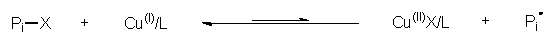
\includegraphics[width=0.7\textwidth]{\figpath/Model1_KATRP_norateconsts}}
	
			Which rate constant determines the length of time for which a radical will stay active before being deactivated?  Based on your answer to part (a), do you expect a higher or lower value of this rate constant to give a better dispersity?
		
		\begin{solution}{}
			$k_{deact}$ determines the amount of time for which a radical will stay active before being deactivated.  A higher value of $k_{deact}$ will give better dispersity because it will result in faster deactivation - i.e. it will ensure that the active radicals are quickly deactivated, and any one active radical does not stay active for too long.
		\end{solution}
			
			\item The equilibrium constant for the ATRP equilibrium shown in part (b) can be written
				\begin{equation*}
					K_{ATRP} = \frac{[\text{Cu}^{(II)}X/L][\text{P}^\bullet]}{[\text{Cu}^{(I)}X/L][\text{PX}]}
				\end{equation*}
				
				Use this information, and appropriate information from Activity 4.\ref{FRPkinetics}, to write an equation for the overall polymerization rate $R_p$ in terms of $K_{ATRP}$, $k_p$, and the concentrations of any relevant chemical species.
		
		\begin{solution}{}
			As shown in Activity 4.\ref{FRPkinetics}, $R_p$ is given by
			\begin{equation*}
				R_p = k_p\text{[M][\ce{P^.}]}
			\end{equation*}
			Rearranging the above expression for $K_{ATRP}$ to solve for $[\text{P}^\bullet]$, we obtain
			\begin{equation*}
				[\text{P}^\bullet] = K_{ATRP}\frac{[\text{Cu}^{(I)}X/L][\text{PX}]}{[\text{Cu}^{(II)}X/L]}
			\end{equation*}
			Combining these two equations, we obtain
			\begin{equation*}
				R_p = k_p\text{[M]}K_{ATRP}\frac{[\text{Cu}^{(I)}X/L][\text{PX}]}{[\text{Cu}^{(II)}X/L]}
			\end{equation*}
		\end{solution}
				
			\item The equilibrium constant for the ATRP equilibrium shown in part (b) can \emph{also} be written as the ratio of the rate constants,
				\begin{equation*}
					K_{ATRP} = \frac{k_{act}}{k_{deact}}
				\end{equation*}
				Substitute this expression into your answer to the previous question to obtain an expression for $R_p$ in terms of $k_{act}$ and $k_{deact}$.
		
		\begin{solution}{}
			\begin{equation*}
				R_p = k_p\text{[M]}\frac{k_{act}}{k_{deact}}\frac{[\text{Cu}^{(I)}X/L][\text{PX}]}{[\text{Cu}^{(II)}X/L]}
			\end{equation*}
		\end{solution}
				
			\item Using your answers to the previous parts of this question, critique or defend the following statement in 2-3 complete sentences:
			
				\emph{``In ATRP, there is often a tradeoff between choosing a catalyst that gives a fast enough polymerization to make a useful amount of polymer, and choosing a catalyst that gives good control over the molecular weight distribution.''}
		
		\begin{solution}{}
			This statement is generally true.  As noted in part (b), obtaining a good dispersity in an ATRP reaction requires a high value for $k_{deact}$.  However, as seen in part (d), a high value of $k_{deact}$ will significantly slow the polymerization.
			
			Note that, typically, increasing $k_{deact}$ decreases the equilibrium constant, so this question gets at the same idea as question \ref{\labelbase:ctq:lowK} in the main activity.  However, it \emph{adds} the criterion that the deactivation rate must itself be high to maintain good control.
		\end{solution}
		
		\end{enumerate}
	
\end{exercises}


%\begin{problems}
%
%	\problem First exercise
%	\problem Second exercise
%	
%\end{problems}


	
\end{activity}